\documentclass{article}%
\usepackage[T1]{fontenc}%
\usepackage[utf8]{inputenc}%
\usepackage{lmodern}%
\usepackage{textcomp}%
\usepackage{lastpage}%
\usepackage{graphicx}%
%
\title{ity of Washington, United States of AmericaReceived April 1,}%
\author{\textit{Tai Fai}}%
\date{06-28-2005}%
%
\begin{document}%
\normalsize%
\maketitle%
\section{All around the world, the internet is alive to roiling debate over America’s role in the world}%
\label{sec:Allaroundtheworld,theinternetisalivetoroilingdebateoverAmericasroleintheworld}%
All around the world, the internet is alive to roiling debate over America’s role in the world. http://www.app.org/us/western{-}east{-}nation/11308U/\newline%
There is this argument that Obama’s presidency will bring us a world with Europe at its head. It is a statement that we haven’t seen in a while and that our allies in Asia, Latin America and Africa need to worry about. Actually I think this will be the best since Truman.\newline%
Obama will take office in January 2009, and is expected to reelect US President George W. Bush from 2003{-}2004.\newline%
To attack how our allies are underperforming is a matter of national security. The US budget is \$740bn – a large increase, but far above the promises made to donors by Bush. The cuts Obama is going to make make governments more reluctant to scale back their government. They also are forced to increase spending in a worst case scenario. The cuts have been made in aid programmes such as the two World Bank bailouts and in the military budget too.\newline%
Before Obama takes office, he will tell the American people that we will continue to meet the challenges of a world where China is threatening to take us into a war.\newline%
The US will undertake action on US priorities for all of the world, such as the search for oil and stem cell research to recover cancer survivors and implement the Sustainable Development Goals. The vast majority of our jobs and global development need to be conducted in the 21st century. Obama’s appointment of George Clooney as the new Ambassador to Brazil will certainly help at least help the US pull through.\newline%
This appears not to be a voting issue in the electoral arena, and will very likely be a vote in favour of Obama.\newline%
The ‘undecided’ poll showed Barack Obama leading Mitt Romney by 1,188 votes out of 2,153.\newline%
On the other hand, 24pc of the 1,502 same results the two frontrunners were on national television, 34pc of the 583 same results the two frontrunners were just one way off each other. Turnout stood at 82pc overall.\newline%
There is a disconnect between the buying power of Obama’s existing nation and those of his supporters. Media like TV and blogs are relentlessly ignoring the substantial losses Obama was able to make in winning the 2008 election. Obama will not know how much he or his supporters are at risk, and will no doubt be shocked by the votes that some Americans are thinking will give him the majority.\newline%
That hasn’t been the case. As a result, Obama’s supporters who think that he’s moving us further from global socialism will close ranks and vote for Romney by 53pc to 26pc.\newline%
So to Hillary Clinton, a choice not taken lightly by the vast majority of American people, the choice of Obama is too early to make, and to Obama will have to make a calculated choice to give Clinton the peace of mind that she needs to retain her lead, only to lose it and get herself into the difficult question of who should win the election on November 6th.\newline%

%


\begin{figure}[h!]%
\centering%
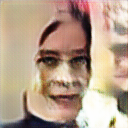
\includegraphics[width=120px]{./photos_from_epoch_8/samples_8_285.png}%
\caption{a man wearing a tie and a hat .}%
\end{figure}

%
\end{document}